\section{Implementazioni utilizzate}
In questa tesi vengono messe a confronto due configurazioni diverse di leggi di contollo che condividono l'algoritmo di trajectory planning. La gestione del percorso non è trattata, vengono definiti per effettuare le simulazione una sequesza di punti nello spazio accompagnati dal tempo alla quale la posizione specifica deve essere raggiunta.
Uno schema generale della configurazione del software dell'autopilota è riportato nella Figura (\ref{fig:Autopilota}).

\begin{figure}
	\centering
	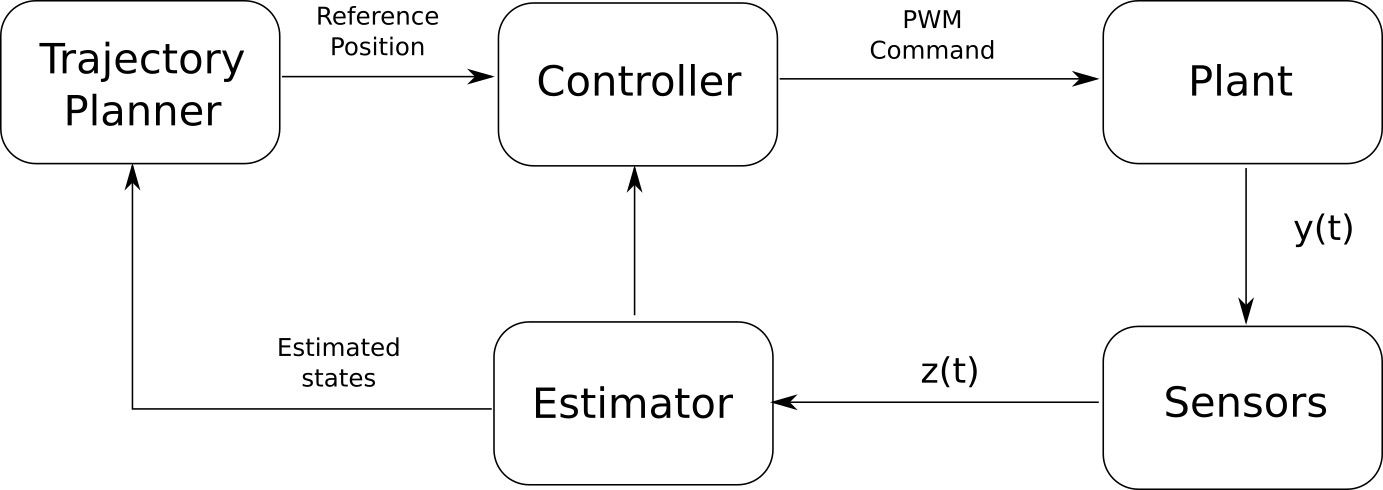
\includegraphics[width=0.6\textwidth]{SistemaQuadrirotore/Figure/Autopilota}
	\caption{Schema della configurazione dell'autopilota}
	\label{fig:Autopilota}
\end{figure}

L'algoritmo implementato per generare la traiettoria è uguale per tutti i tipi di simulazioni che sono state fatte. Data una sequenza di punti espressi in termini di coordinate nello spazio e il tempo rispetto all'inizio della simulazione per raggiungimento di tale punto, viene definita una legge della traiettoria con profilo di velocità a forma trapezoidale, utilizzando come vincolo la velocità massima posta a $g/2$, \cite{DesTestCarm}.

Sia nelle simulazioni MIL e SIL due tipologie di controllori vengono messi a confronto. In entrambe le configurazioni il controllore viene suddiviso in tre componenti base: Altitude Controller, Attitude Controller e Position Controller, come mostrato in Figura (\ref{fig:Controller}).


\begin{figure}
	\centering
	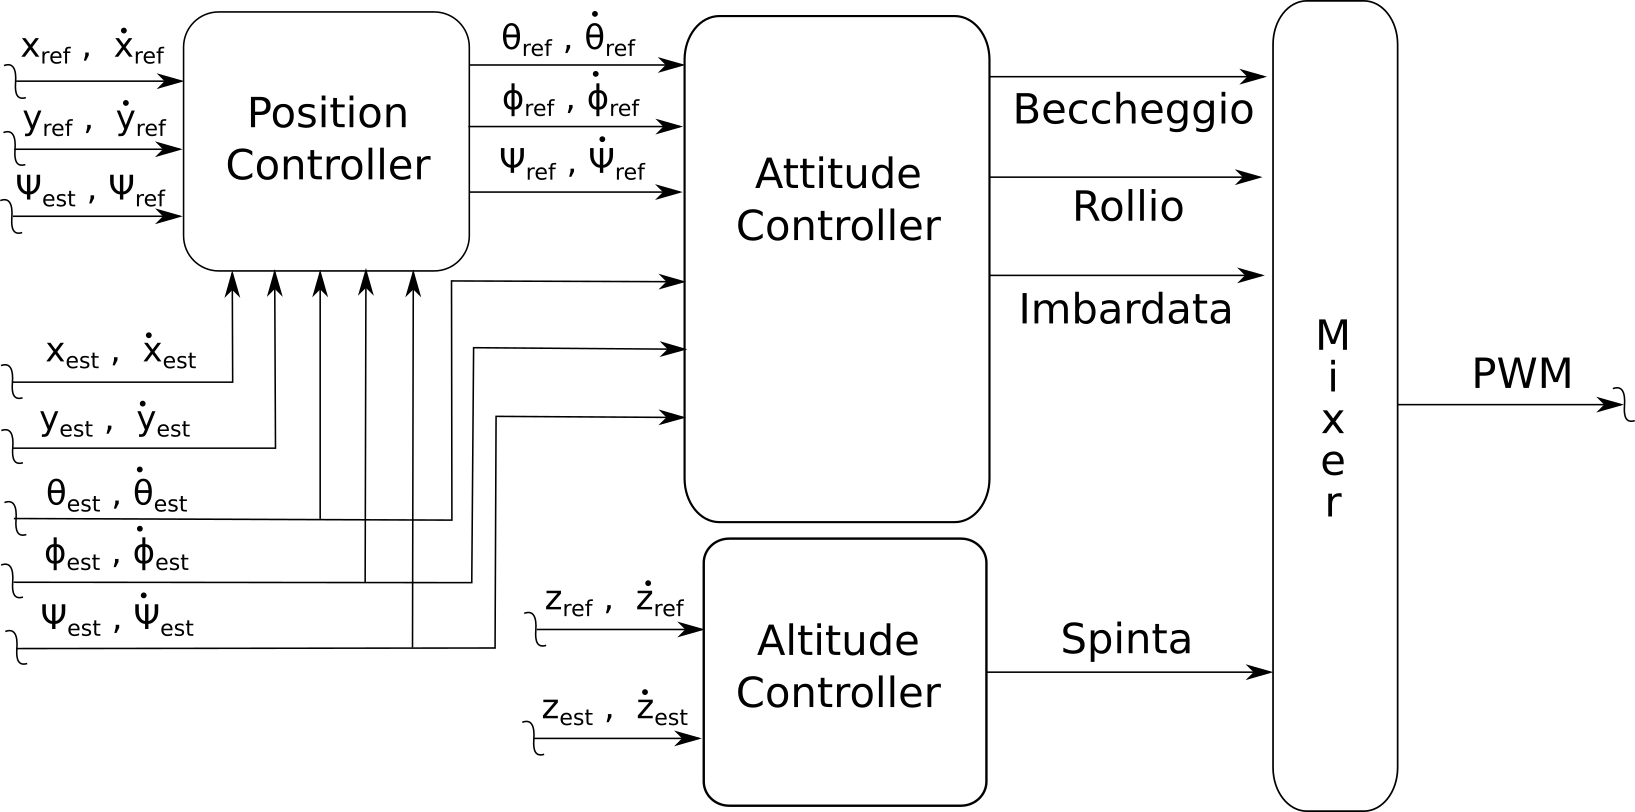
\includegraphics[width=0.7\textwidth]{SistemaQuadrirotore/Figure/Controllore}
	\caption{Schema della configurazione del software dell'autopilota}
	\label{fig:Controller}
\end{figure}